% Full project hour tracking appendix generated from TimelisteBachelor2026.xlsx
% Recommended packages in the preamble:
% \usepackage{booktabs}
% \usepackage{longtable}
% \usepackage{array}
% \usepackage{graphicx}
% \usepackage{float}

\chapter{Project Hour Tracking}
\label{app:project-hour-tracking}
\raggedbottom

This appendix presents the project hour tracking maintained throughout the bachelor project. The hour list was used to document weekly work distribution across planning, meetings, documentation, programming, testing, research, figures, and administration. The appendix first presents a condensed overview of the total work distribution, followed by the complete weekly hour logs from the original spreadsheet.

\section{Condensed Overview}
\label{appendix:project-hour-tracking-overview}

\begin{table}[htbp]
\centering
\caption{Total registered project hours by group member.}
\label{tab:project-hours-member-total}
\begin{tabular}{lr}
\toprule
Group member & Total hours \\
\midrule
Hoang & 723 \\
Henrik & 674 \\
Karwan & 788.5 \\
\midrule
Total & 2185.5 \\
\bottomrule
\end{tabular}
\end{table}

\begin{table}[htbp]
\centering
\caption{Total registered project hours by activity category.}
\label{tab:project-hours-category-total}
\begin{tabular}{lr}
\toprule
Activity category & Total hours \\
\midrule
Programming & 729 \\
Report documentation & 579 \\
Planning and meetings & 309 \\
Research & 254 \\
Testing & 104 \\
Git and administration & 103.5 \\
Figures and diagrams & 63.5 \\
Code documentation & 43.5 \\
\midrule
Total & 2185.5 \\
\bottomrule
\end{tabular}
\end{table}

\begin{figure}[htbp]
    \centering
    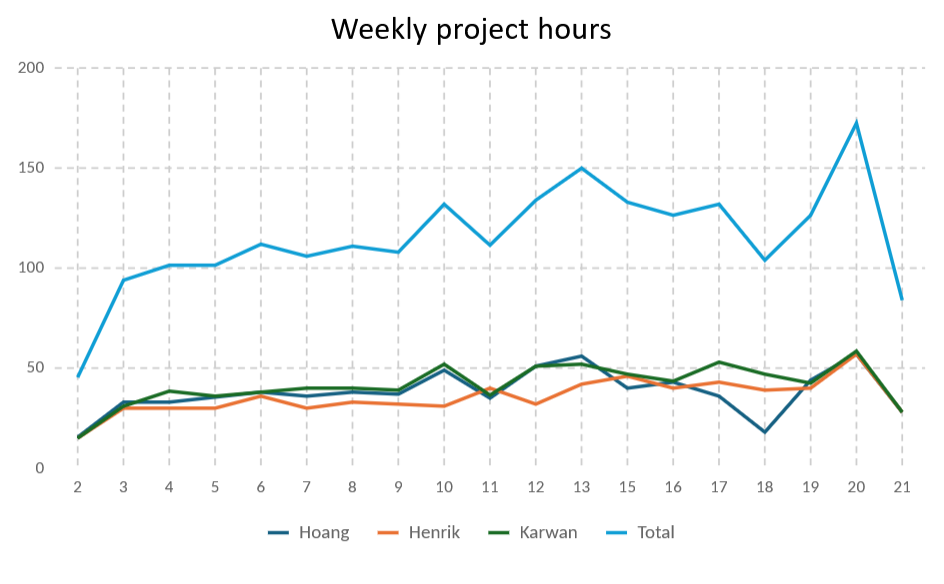
\includegraphics[width=0.85\textwidth]{figures/images/chapter-3/project_hours_weekly_summary_user_chart.png}
    \caption{Summary of registered project hours across the project period.}
    \label{fig:project-hours-weekly-summary}
\end{figure}

\begin{figure}[htbp]
    \centering
    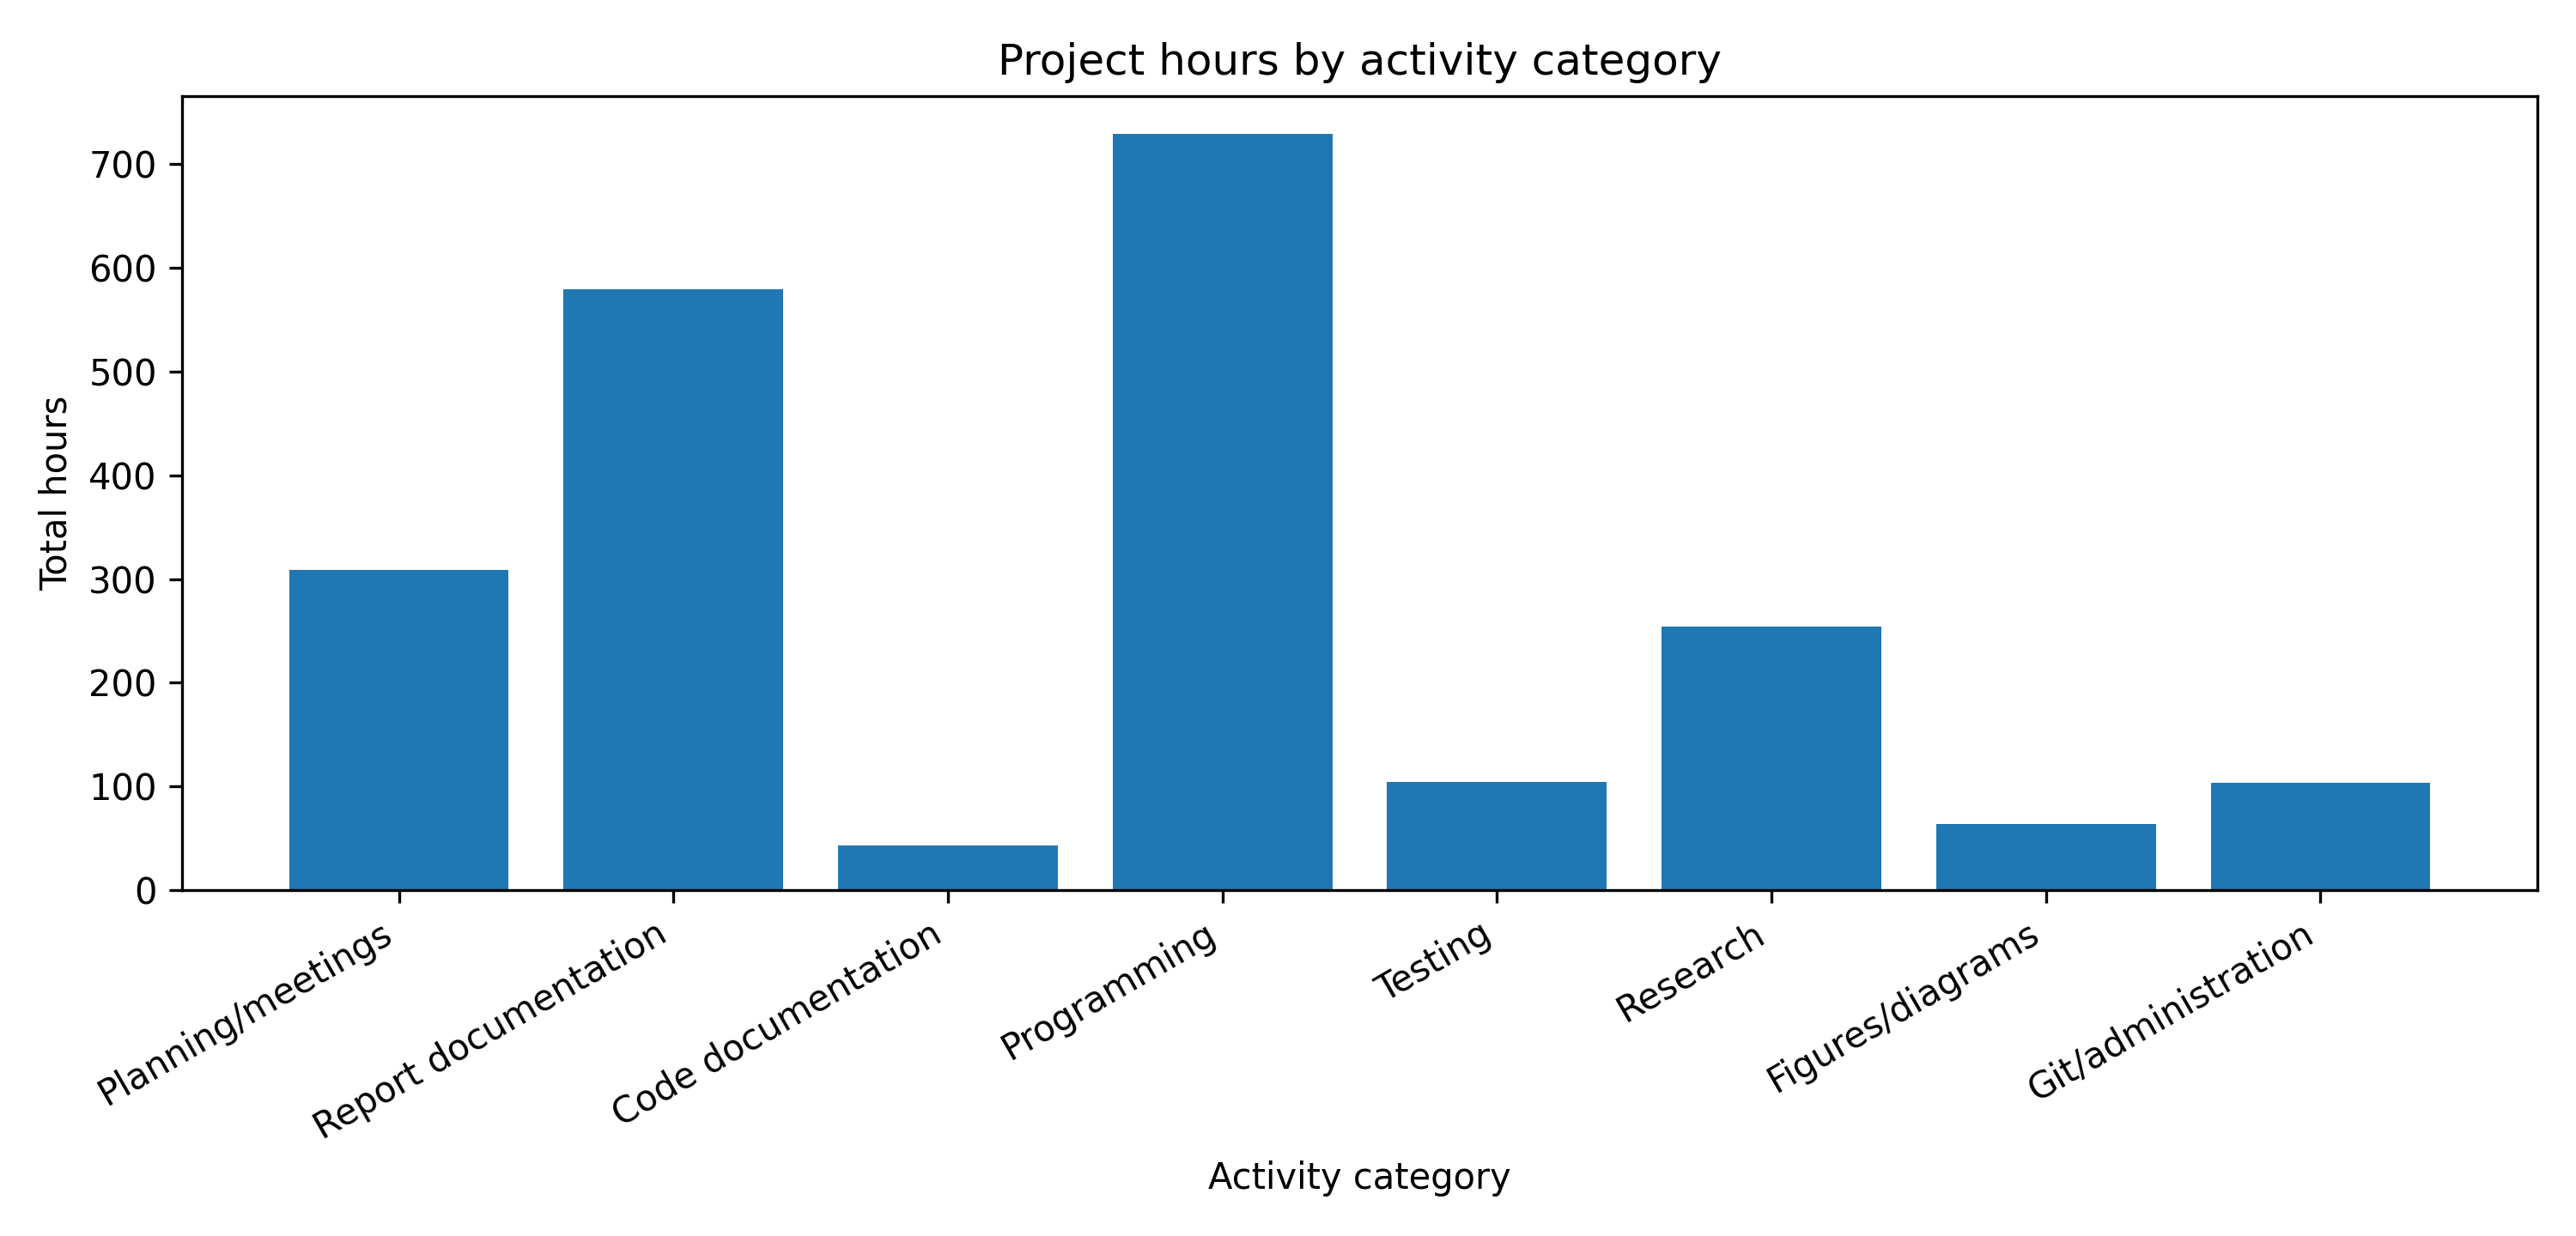
\includegraphics[width=0.80\textwidth]{figures/images/chapter-3/project_hours_category_summary.png}
    \caption{Distribution of registered project hours by activity category.}
    \label{fig:project-hours-category-summary}
\end{figure}

\begin{longtable}{lrrrr}
\caption{Weekly registered project hours by group member.}
\label{tab:project-hours-weekly-overview}\\
\toprule
Week & Hoang & Henrik & Karwan & Total \\
\midrule
\endfirsthead
\toprule
Week & Hoang & Henrik & Karwan & Total \\
\midrule
\endhead
Uke2 & 15.5 & 15 & 15 & 45.5 \\
Uke3 & 33 & 30 & 31 & 94 \\
Uke4 & 33 & 30 & 38.5 & 101.5 \\
Uke5 & 35.5 & 30 & 36 & 101.5 \\
Uke6 & 38 & 36 & 38 & 112 \\
Uke7 & 36 & 30 & 40 & 106 \\
Uke8 & 38 & 33 & 40 & 111 \\
Uke9 & 37 & 32 & 39 & 108 \\
Uke10 & 49 & 31 & 52 & 132 \\
Uke11 & 35 & 40 & 36.5 & 111.5 \\
Uke12 & 51 & 32 & 51 & 134 \\
Uke13 & 56 & 42 & 52 & 150 \\
Uke15 & 40 & 46 & 47 & 133 \\
Uke16 & 43 & 40 & 43.5 & 126.5 \\
Uke17 & 36 & 43 & 53 & 132 \\
Uke18 & 18 & 39 & 47 & 104 \\
Uke19 & 44 & 40 & 42.5 & 126.5 \\
Uke20 & 57 & 57 & 58.5 & 172.5 \\
Uke21 & 28 & 28 & 28 & 84 \\
\midrule
Total & 723 & 674 & 788.5 & 2185.5 \\
\bottomrule
\end{longtable}

\section{Complete Weekly Hour Logs}
\label{appendix:project-hour-tracking-complete}

The following tables reproduce the complete weekly hour logs from the project hour list. Each week includes the registered hours by activity category and group member. When the spreadsheet included written comments, these are included below the corresponding weekly hour table.

\subsection{Uke2}

\begin{table}[H]
\centering
\small
\caption{Registered hours for Uke2.}
\label{tab:project-hours-uke2}
\begin{tabular}{lrrrr}
\toprule
Activity & Hoang & Henrik & Karwan & Total \\
\midrule
Møter & 4 & 4 & 4 & 12 \\
Dokumentasjon - Rapport & 5 & 6 & 5 & 16 \\
Dokumentasjon - Kode & 0 & 0 & 0 & 0 \\
Programmering & 0 & 0 & 0 & 0 \\
Testing & 0 & 0 & 0 & 0 \\
Forskning & 4 & 2 & 3 & 9 \\
Figurer og diagrammer & 0.5 & 1.5 & 1 & 3 \\
Git / Administrasjon & 2 & 1.5 & 2 & 5.5 \\
\midrule
Total & 15.5 & 15 & 15 & 45.5 \\
\bottomrule
\end{tabular}
\end{table}

\begin{longtable}{p{0.20\textwidth}p{0.72\textwidth}}
\caption{Written activity notes for Uke2.}\\
\toprule
Entry & Notes \\
\midrule
\endfirsthead
\toprule
Entry & Notes \\
\midrule
\endhead
Hoang & Satte opp GitLab Kanban tavle og excel dokumentet. \newline Tok kontakt med OsloSkolen for mulig samarbeid. \newline Satte opp gruppe kontrakt og fikk signaturer. \newline Ansvar for kapittel en og tre for prosjektplanen. \\
\addlinespace
Henrik & Har skrevet punkt 4 om planlegging, oppfølging og rapportering. Har skrevet møtereferater og satt opp online møter. Har laget kanaler hvor vi kan snakke sammen og dele felles dokumenter/organisere ting vi har diskutert etter tema slik at vi lett kan finne fram og være oppdatert. Har utforsket teori om oppgaven. \\
\addlinespace
Karwan & Forskning: Forbredelse ved å lese tidligere bachleor oppgaver. Møter: Henvend til møtereferatene fra uke 2. Rapportering: Skrive "Organisering og Kvalitetssikring" og analysere risiko. Kontakte ulike bedrifter for mulige bachleor oppgaver. \\
\addlinespace
\bottomrule
\end{longtable}

\subsection{Uke3}

\begin{table}[H]
\centering
\small
\caption{Registered hours for Uke3.}
\label{tab:project-hours-uke3}
\begin{tabular}{lrrrr}
\toprule
Activity & Hoang & Henrik & Karwan & Total \\
\midrule
Møter & 7 & 8 & 7 & 22 \\
Dokumentasjon - Rapport & 9 & 6 & 7 & 22 \\
Dokumentasjon - Kode & 0 & 0 & 0 & 0 \\
Programmering & 0 & 0 & 0 & 0 \\
Testing & 0 & 0 & 0 & 0 \\
Forskning & 10 & 6 & 14 & 30 \\
Figurer og diagrammer & 1 & 6 & 2 & 9 \\
Git / Administrasjon & 6 & 4 & 1 & 11 \\
\midrule
Total & 33 & 30 & 31 & 94 \\
\bottomrule
\end{tabular}
\end{table}

\begin{longtable}{p{0.20\textwidth}p{0.72\textwidth}}
\caption{Written activity notes for Uke3.}\\
\toprule
Entry & Notes \\
\midrule
\endfirsthead
\toprule
Entry & Notes \\
\midrule
\endhead
Hoang & Bearbeidet prosjektplanen, og har sett på en del research angående sladding av sensitiv informasjon på bilder, hvordan andre modeller har gjort det kontra våres potensiell løsnign. Har også gjort en del research om react rammeverket og hvordan det brukes for å lage nettsider, I tillegg til å eksperimentere med rammeverket. Har også satt opp GitHub og Jira, og vurdert hvilken kanban tavle som er best (kollektivt). Opprettet frontend prosjektet og initialisert til GitHub. \\
\addlinespace
Henrik & Jobbet videre med prosjektplanen. Skrevet møtereferater og notert på møter. Oppsummert møter og vært scrum ansvarlig. Kommet på ideer til løsninger. Bidrat til spørsmål til oppdragsgiver/rådgiver. Laget Gantt skjema og kommet på plan for prosjektets tidslinje. Hjulpet med å komme på løsning til administrasjon og sette opp Jira. \\
\addlinespace
Karwan & Bruke tid på å se etter eksisterende løsninger innen ansiktdjenskjenning og ansiktsdetection. Se etter modeller som kan brukes i prosjektet. Lese teori innen maskin læring. Teste disse ulike eksisterende løsningene på python og se om det er noe å ta med. Pusse opp omfang delen i prosjekt rapporten. Fikse Wiki page for GitHub. \\
\addlinespace
\bottomrule
\end{longtable}

\subsection{Uke4}

\begin{table}[H]
\centering
\small
\caption{Registered hours for Uke4.}
\label{tab:project-hours-uke4}
\begin{tabular}{lrrrr}
\toprule
Activity & Hoang & Henrik & Karwan & Total \\
\midrule
Møter & 7 & 8 & 7 & 22 \\
Dokumentasjon - Rapport & 4 & 5 & 4 & 13 \\
Dokumentasjon - Kode & 0 & 0 & 1 & 1 \\
Programmering & 17 & 0 & 20 & 37 \\
Testing & 0 & 0 & 2 & 2 \\
Forskning & 3 & 10 & 4 & 17 \\
Figurer og diagrammer & 0 & 2 & 0.5 & 2.5 \\
Git / Administrasjon & 2 & 5 & 0 & 7 \\
\midrule
Total & 33 & 30 & 38.5 & 101.5 \\
\bottomrule
\end{tabular}
\end{table}

\begin{longtable}{p{0.20\textwidth}p{0.72\textwidth}}
\caption{Written activity notes for Uke4.}\\
\toprule
Entry & Notes \\
\midrule
\endfirsthead
\toprule
Entry & Notes \\
\midrule
\endhead
Hoang & Brukt meste av tiden til å utvikle en prototype som skal bli kastet på react + vite i tillegg til litt research om best practices innen for dem. Fått til en enkel nettside med enkel redigering. Redigert litt på prosjektplanen etter tilbakemelding fra veileder og passe på at språket er mer konsistent. \\
\addlinespace
Henrik & Ferdigstillte prosjektrapport. Fant state of the art av image preprocessing for facedetection, object detection og character detection. Researchet hva som menes med sensitiv informasjon/hva som brukes i praksis. Skrev møtereferater, passet på at scrum ble fulgt. \\
\addlinespace
Karwan & Research innen face recognition og face detection. Finne modeller som gir gode resultater. Testing for å gjøre disse modellene bedre. Vi valgte RetinaFace for å finne ansikter i bilder, for den er den største modellen og som gir veldig gode resultater, både av små ansikter (distanse ) og gruppe bilder. Retina er dårlig på å finne ansikter som ikke vises fult (f.eks hjelm, maske, osv), la til augmentasjion + occulation for å gjøre modellen bedre. Bruker YOLO for å finne fulle kropper og ikke bare ansikter. Evaluere modellene, sammenligne fine tuned modell med base modellen. \\
\addlinespace
\bottomrule
\end{longtable}

\subsection{Uke5}

\begin{table}[H]
\centering
\small
\caption{Registered hours for Uke5.}
\label{tab:project-hours-uke5}
\begin{tabular}{lrrrr}
\toprule
Activity & Hoang & Henrik & Karwan & Total \\
\midrule
Møter & 5 & 6 & 5 & 16 \\
Dokumentasjon - Rapport & 4 & 1 & 1 & 6 \\
Dokumentasjon - Kode & 3 & 0 & 1 & 4 \\
Programmering - Front & 18 & 0 & 0 & 18 \\
Programmering - Back & 0 & 7 & 19 & 26 \\
Testing & 1 & 1 & 1 & 3 \\
Forskning & 2 & 13 & 8 & 23 \\
Figurer og diagrammer & 0.5 & 1 & 0 & 1.5 \\
Git / Administrasjon & 2 & 1 & 1 & 4 \\
\midrule
Total & 35.5 & 30 & 36 & 101.5 \\
\bottomrule
\end{tabular}
\end{table}

\begin{longtable}{p{0.20\textwidth}p{0.72\textwidth}}
\caption{Written activity notes for Uke5.}\\
\toprule
Entry & Notes \\
\midrule
\endfirsthead
\toprule
Entry & Notes \\
\midrule
\endhead
Hoang & Skrev siste endringer (GDPR og regler) på prosjektplan etter møte med oppdragsgiver, samtidig som tankekartet ble revidert. La til manuell sladding i frontend samtidig enkle funksjonalitet som å laste ned filen og zoome in og ut på bildet. Protoypen ble refaktorert og satt inn i MVP repo. Dokumentasjon for klassene ble lagt til, kompleks logikk fikk kommentarer. Sett bittelitt på hvordan GitHub Actions fungerer og satt det opp. \\
\addlinespace
Henrik & Researchet/laget og testet kode for preprocessing av bilder opp mot retinaface-modellen. Hvilke threshholds/hva slags preprocessing gjør at modellen klarer å finne flest ansikter i en folkemengde. Hva fungerer best på bilder med forskjellig stø. Hva vil være beste metode med tanke på tid modellen bruker. Dersom vi skal legge til tekst i framtiden, hva slags preprocessing gjøres for å detektere områder der tekst mest sannsynlig ligger i bildet. Skrevet på rapport. Endret på Gannt skjema. \\
\addlinespace
Karwan & Finpusse prosjektplan rapporten. Gå gjennom for å bekrefte den før levering. Implementere pipeline for backend slik at den kan senere bli brukt av frontend. Implementere API, og ulike endepunkter for å sende informasjon. Fine-tune retinaface modellen for å se om vi kan gjøre den bedre enn base modellen. \\
\addlinespace
\bottomrule
\end{longtable}

\subsection{Uke6}

\begin{table}[H]
\centering
\small
\caption{Registered hours for Uke6.}
\label{tab:project-hours-uke6}
\begin{tabular}{lrrrr}
\toprule
Activity & Hoang & Henrik & Karwan & Total \\
\midrule
Oppgave Tema & 0 & 0 & 0 & 0 \\
Planlegging/Møter & 5 & 6 & 5 & 16 \\
Dokumentasjon - Rapport & 0 & 6 & 0 & 6 \\
Dokumentasjon - Kode & 3 & 0 & 2 & 5 \\
Programmering - Front & 26 & 0 & 2 & 28 \\
Programmering - Back & 0 & 13 & 25 & 38 \\
Testing & 0 & 0 & 1 & 1 \\
Forskning & 2 & 10 & 2 & 14 \\
Figurer og diagrammer & 0 & 0 & 0 & 0 \\
Git / Administrasjon & 2 & 1 & 1 & 4 \\
\midrule
Total & 38 & 36 & 38 & 112 \\
\bottomrule
\end{tabular}
\end{table}

\begin{longtable}{p{0.20\textwidth}p{0.72\textwidth}}
\caption{Written activity notes for Uke6.}\\
\toprule
Entry & Notes \\
\midrule
\endfirsthead
\toprule
Entry & Notes \\
\midrule
\endhead
Hoang & Riktig skalering på knapper og komponenter avhengig av vindu størrelse er nå implementert. Lagt til andre UI/UX elementer som kan hjelpe bruker opplevelsen. PDF er nå redigerbar. Prøvd å refaktorere koden, men må jobbes mer med. Har satt opp inndeling for prosjekt rapporten. \\
\addlinespace
Henrik & Har jobbet med segmentation av personer i bildene i backend. Har gjort forskning på gdpr, state of the art og så vidt begynt på rapporten for kapittel 2. \\
\addlinespace
Karwan & Optimalisere hastigheten til redaction av ansikter, for redaction var unødvendig treig. Gi mulighet til brukeren slik at de kan velge ut hva slags ansikter de ikke vil redacte. Gjøre anonymisering sterkere. Bruke Go som offisiel språk for API. Rydde og refaktorisere koden slik at det er ryddig, legge til dokumentasjon. \\
\addlinespace
\bottomrule
\end{longtable}

\subsection{Uke7}

\begin{table}[H]
\centering
\small
\caption{Registered hours for Uke7.}
\label{tab:project-hours-uke7}
\begin{tabular}{lrrrr}
\toprule
Activity & Hoang & Henrik & Karwan & Total \\
\midrule
Planlegging/Møter & 5 & 6 & 5 & 16 \\
Dokumentasjon - Rapport & 14 & 8 & 0 & 22 \\
Dokumentasjon - Kode & 0 & 0 & 1 & 1 \\
Programmering - Front & 2 & 0 & 10 & 12 \\
Programmering - Back & 0 & 0 & 12 & 12 \\
Testing & 0 & 0 & 5 & 5 \\
Forskning & 9 & 14 & 5 & 28 \\
Figurer og diagrammer & 2 & 0 & 0 & 2 \\
Git / Administrasjon & 4 & 2 & 2 & 8 \\
\midrule
Total & 36 & 30 & 40 & 106 \\
\bottomrule
\end{tabular}
\end{table}

\begin{longtable}{p{0.20\textwidth}p{0.72\textwidth}}
\caption{Written activity notes for Uke7.}\\
\toprule
Entry & Notes \\
\midrule
\endfirsthead
\toprule
Entry & Notes \\
\midrule
\endhead
Hoang & Inndelte kapitlene enda mer I overleaf for å lage grov oversikt over hva som skal med, basert på tidligere bachelor oppgaver. Startet med første chapter for bachelor oppgavene, altså om oppgavebeskrivelsen, mål, rammer, osv. Gjorde en del research om lignende oppgaver og om modeller som kan brukes for tekst og om lisenser som trengs. I tillegg lest en del bachelor oppgaver for å få helhetelig bildet på hvordan våres skal se ut. \\
\addlinespace
Henrik & Har researchet gdpr, state of art, begynt på rapporten og sett på mulige løsninger for videreutvikling av koden. \\
\addlinespace
Karwan & Refaktorere koden til frontend og backend. Ridde opp dokumentasjoner, dele opp koden. Refaktorere mappe struktur. Fikse bugs, blant annent som synkronisere manuel redaction med automatisk redaction. Gjøre hastigheten til redaction bedre. Legge til CRAFT (tekst deteksjon) til backend og koble den til frontend. Forskning innen ulike modeller for tekstdeteksjon innen bilder. \\
\addlinespace
\bottomrule
\end{longtable}

\subsection{Uke8}

\begin{table}[H]
\centering
\small
\caption{Registered hours for Uke8.}
\label{tab:project-hours-uke8}
\begin{tabular}{lrrrr}
\toprule
Activity & Hoang & Henrik & Karwan & Total \\
\midrule
Planlegging/Møter & 5 & 6 & 5 & 16 \\
Dokumentasjon - Rapport & 6 & 0 & 0 & 6 \\
Dokumentasjon - Kode & 1 & 0 & 1 & 2 \\
Programmering - Front & 14 & 10 & 2 & 26 \\
Programmering - Back & 0 & 8 & 23 & 31 \\
Programmering - Bugs & 5 & 2 & 1 & 8 \\
Testing & 0 & 0 & 3 & 3 \\
Forskning & 4 & 5 & 3 & 12 \\
Figurer og diagrammer & 0 & 0 & 1 & 1 \\
Git / Administrasjon & 3 & 2 & 1 & 6 \\
\midrule
Total & 38 & 33 & 40 & 111 \\
\bottomrule
\end{tabular}
\end{table}

\begin{longtable}{p{0.20\textwidth}p{0.72\textwidth}}
\caption{Written activity notes for Uke8.}\\
\toprule
Entry & Notes \\
\midrule
\endfirsthead
\toprule
Entry & Notes \\
\midrule
\endhead
Hoang & Prøvd å ta litt kontakt med ulike potenseille bruketestere som for eksempel fra NRK eller VG. Brukt tid på å legge til bruke innstillinger I applikasjonen vår, I tillegg til å fikse noen bugs. Har satt opp overleaf dokumentet etter ntnu sine standarder og holder på å overføre tekst fra den gamle. Gjort litt mer forksning på the state of art. \\
\addlinespace
Henrik & Jobbet med downscaling methods i backend. Fikset terms of service i frontend. Lagde to forskjellige brukertester, en tilpasset testing for funksjonalitet og en for UI. \\
\addlinespace
Karwan & Fjerne PDF støtte pga ikke lenger behov, forenkle frontend for kunn bilde støtte. Teste alle ende punkter (redact\&detect) og sørge for at de fungerer. Dekke så mye av backend koden som mulig med unit testing. Legge til script for å starte frontend og backend enkelt samtidig (loklat). Contrainerize backend med docker. Fikse Google Cloud Run for å kunne deploye applikasjonen. Legge til dokumenatison i koden. Evaluere retinaface modelene (resnet50 og mobilnet\_25) for rapport og prøve å fine tune den. \\
\addlinespace
\bottomrule
\end{longtable}

\subsection{Uke9}

\begin{table}[H]
\centering
\small
\caption{Registered hours for Uke9.}
\label{tab:project-hours-uke9}
\begin{tabular}{lrrrr}
\toprule
Activity & Hoang & Henrik & Karwan & Total \\
\midrule
Planlegging/Møter & 5 & 6 & 5 & 16 \\
Dokumentasjon - Rapport & 3 & 0 & 0 & 3 \\
Dokumentasjon - Kode & 1 & 0 & 1 & 2 \\
Programmering - Front & 21 & 0 & 10 & 31 \\
Programmering - Back & 0 & 7 & 15 & 22 \\
Programmering - Bugs & 0 & 0 & 5 & 5 \\
Testing & 2 & 9 & 1 & 12 \\
Forskning & 4 & 4 & 1 & 9 \\
Figurer og diagrammer & 0 & 3 & 0 & 3 \\
Git / Administrasjon & 1 & 3 & 1 & 5 \\
\midrule
Total & 37 & 32 & 39 & 108 \\
\bottomrule
\end{tabular}
\end{table}

\begin{longtable}{p{0.20\textwidth}p{0.72\textwidth}}
\caption{Written activity notes for Uke9.}\\
\toprule
Entry & Notes \\
\midrule
\endfirsthead
\toprule
Entry & Notes \\
\midrule
\endhead
Hoang & La til ulike UI/UX funksjonaliteter som for eksempel farge endring, filtere og brukerpreferanser. Har startet med å legge til noe support for video og videoformatering. Gjort research på hvordan tidligere prosjekter/andre bedrifter og firmaer og gjort denne løsningen. Forbedret biter fra chapter 1 fra det gamle overleaf dokumentet. Har også sett på standarder innen for testing og hvordan testing skal være, i tillegg til å lage nye test filer og oppdatere den gamle test filen. \\
\addlinespace
Henrik & Tok kontakt med firmaer for brukertesting. Lagde funksjon for å få bounding boxes fra video ved bruk av tracking. Testet alle mulige API calls lokalt og via nettsiden, fra powershell og inspector tools, for å se hvor performance går tapt. Samlet dataen og lagde simple tabeller for dette. Fikk en oversikt over pipeline og hva som gjør at vi mister performance underveis der (benchmarking). \\
\addlinespace
Karwan & Fikse bugger fra applikasjonen. Utforske andre tekst deteksjons modeller som er bedre enn CRAFT. Bytte teks deteksjon fra CRAFT til PaddleOCR. Oppdatere tester. Legge til tekst analyse etter tekst deteksjon for å kunne filtrere de ut (om det er noe sensetiv info., som tlf. nummer, bil skylt, post nummer, osv.). Koble filtrering funsksjonalitet til frontend. Refaktorere frontend. Legge til QR-Bar -Detection. \\
\addlinespace
\bottomrule
\end{longtable}

\subsection{Uke10}

\begin{table}[H]
\centering
\small
\caption{Registered hours for Uke10.}
\label{tab:project-hours-uke10}
\begin{tabular}{lrrrr}
\toprule
Activity & Hoang & Henrik & Karwan & Total \\
\midrule
Planlegging/Møter & 5 & 6 & 5 & 16 \\
Dokumentasjon - Rapport & 11 & 0 & 12 & 23 \\
Dokumentasjon - Kode & 1 & 0 & 1 & 2 \\
Programmering - Front & 3 & 0 & 2 & 5 \\
Programmering - Back & 0 & 13 & 10 & 23 \\
Programmering - Bugs & 11 & 0 & 10 & 21 \\
Testing & 6 & 4 & 2 & 12 \\
Forskning & 8 & 0 & 5 & 13 \\
Figurer og diagrammer & 1 & 0 & 4 & 5 \\
Git / Administrasjon & 3 & 8 & 1 & 12 \\
\midrule
Total & 49 & 31 & 52 & 132 \\
\bottomrule
\end{tabular}
\end{table}

\begin{longtable}{p{0.20\textwidth}p{0.72\textwidth}}
\caption{Written activity notes for Uke10.}\\
\toprule
Entry & Notes \\
\midrule
\endfirsthead
\toprule
Entry & Notes \\
\midrule
\endhead
Hoang & Testere for utils og hooks samtidig integrasjons tests ble laget. Ordnet mer på overleaf dokumentet sin fil struktur og pakker, samtidig ble det hentet frem/laget nye figurer for kapitell 6. Har startet å skrive på kapittel 6 og kapittel 1 har blitt revidert utifra tilbakemleding fra veileder. Prøvd å fikse fleste bugs fra kanalen vår og lagt til en drag feature for når man er zoomed langt inn på canvas. \\
\addlinespace
Henrik & Har hold kontakt med bedrifter for brukertesting. Har fått video til å fungere med redact, og endret struktur og logikk slik at det skal være lett å koble det opp med siden vår. \\
\addlinespace
Karwan & Utforsket ulike modeller vi kan finetune for licensplate og barcode deteksjon. YOLOX var den som fylte alle kravene (lisens, gratis og bra). Samlet inn data for barcode, brukte mye tid på å finne dataset, kombinerte fra ulike kilder. Deretter finpusset (fjerne duplikater, bilder uten labels, osv) og splittet jeg datasettet og gjorde det klar for trening. Trente modellen og andre modeller med ulike parametere, samlet data også lagde jeg figurer for evalueringer. Brukte disse da til rapporten, og skrev i kappitel 8 og 13. Implemnterte beste modellen for barcode inn i systemet, og debugget til alt fungerte. \\
\addlinespace
\bottomrule
\end{longtable}

\subsection{Uke11}

\begin{table}[H]
\centering
\small
\caption{Registered hours for Uke11.}
\label{tab:project-hours-uke11}
\begin{tabular}{lrrrr}
\toprule
Activity & Hoang & Henrik & Karwan & Total \\
\midrule
Planlegging/Møter & 8 & 9 & 5 & 22 \\
Dokumentasjon - Rapport & 0 & 0 & 2 & 2 \\
Dokumentasjon - Kode & 1 & 0 & 0.5 & 1.5 \\
Programmering - Front & 4 & 0 & 0 & 4 \\
Programmering - Back & 0 & 8 & 15 & 23 \\
Programmering - Bugs & 10 & 0 & 3 & 13 \\
Testing & 1 & 0 & 2 & 3 \\
Forskning & 5 & 15 & 2 & 22 \\
Figurer og diagrammer & 0 & 0 & 2 & 2 \\
Git / Administrasjon & 6 & 8 & 5 & 19 \\
\midrule
Total & 35 & 40 & 36.5 & 111.5 \\
\bottomrule
\end{tabular}
\end{table}

\begin{longtable}{p{0.20\textwidth}p{0.72\textwidth}}
\caption{Written activity notes for Uke11.}\\
\toprule
Entry & Notes \\
\midrule
\endfirsthead
\toprule
Entry & Notes \\
\midrule
\endhead
Hoang & Forbrede til møte og jobbet med å få til en fungerende versjon for deployment til møte med skan kontroll. Gjorde litt forskning på metadata og hvordan undersøke om et bildet er legitimt eller laget av kunstig intelligens. Etter rell behov. Også litt research på hvordan man får maksimal utbytte av brukertesting. \\
\addlinespace
Henrik & Forbrede til møte med skan kontroll og delta på møtet. Jobbet også med videoimplementasjon og gjorde research på kalman filter og annet video tracking muligheter. \\
\addlinespace
Karwan & Jobbet med YOLOX/data module og requrments. Trente YOLOX-S license plate deteksjons modell. Evaluerte modellen, lagde oversiktlig evaluerings grafer og skrev resultat analyse for rapporten. Implementerte modellen inn i SafeVision backend systemet. Fikset Docker, Cloud Run, model preload. Fikse på CI/CD problemer (modeller blir ikke lastet til google cloude). Fikset bounding boxes for skilt ved scaling mismatch. \\
\addlinespace
\bottomrule
\end{longtable}

\subsection{Uke12}

\begin{table}[H]
\centering
\small
\caption{Registered hours for Uke12.}
\label{tab:project-hours-uke12}
\begin{tabular}{lrrrr}
\toprule
Activity & Hoang & Henrik & Karwan & Total \\
\midrule
Planlegging/Møter & 7 & 8 & 5 & 20 \\
Dokumentasjon - Rapport & 9 & 0 & 0 & 9 \\
Dokumentasjon - Kode & 1 & 0 & 5 & 6 \\
Programmering - Front & 18 & 0 & 2 & 20 \\
Programmering - Back & 0 & 20 & 25 & 45 \\
Programmering - Bugs & 5 & 0 & 5 & 10 \\
Testing & 2 & 0 & 3 & 5 \\
Forskning & 5 & 3 & 1 & 9 \\
Figurer og diagrammer & 3 & 0 & 0 & 3 \\
Git / Administrasjon & 1 & 1 & 5 & 7 \\
\midrule
Total & 51 & 32 & 51 & 134 \\
\bottomrule
\end{tabular}
\end{table}

\begin{longtable}{p{0.20\textwidth}p{0.72\textwidth}}
\caption{Written activity notes for Uke12.}\\
\toprule
Entry & Notes \\
\midrule
\endfirsthead
\toprule
Entry & Notes \\
\midrule
\endhead
Hoang & Møte med Thomas Berg Fjellestad som er studieprogramleder og universitetslektor ga informasjon om hvordan få mer ut av brukertesting og annet teori rundt det. I tillegg litt feedback på UI/UX designet vårt. Prøvde å få til metadata inn til frontenden, men bestemte for å kutte det ut. La til tooltips og labels for å gjøre det lettere å navigere rundt UI/UX. Har også gjort om ID fra number til Strings. Ny funksjonalitet er høyreklikk og highlights på bokser for å indikere at de er selected. Skrevet noe i chapter 3 i rapporten. Og revidert litt utifra tilbakemelding fra veileder. \\
\addlinespace
Henrik & Jobbet med videoimplementasjon, forbredet og deltok på møte om brukertesting og UI design \\
\addlinespace
Karwan & La til concurrency i detect/redact pipelines. Utvidet detection pipeline med objekt-detection, categories og entities. Fikset redaction box masking og single-pass anonymization. Oppdaterte dokumentasjon. Rettet CI- og ruff-feil. \\
\addlinespace
\bottomrule
\end{longtable}

\subsection{Uke13}

\begin{table}[H]
\centering
\small
\caption{Registered hours for Uke13.}
\label{tab:project-hours-uke13}
\begin{tabular}{lrrrr}
\toprule
Activity & Hoang & Henrik & Karwan & Total \\
\midrule
Planlegging/Møter & 5 & 6 & 5 & 16 \\
Dokumentasjon - Rapport & 25 & 6 & 0 & 31 \\
Dokumentasjon - Kode & 1 & 1 & 2 & 4 \\
Programmering - Front & 12 & 4 & 8 & 24 \\
Programmering - Back & 0 & 12 & 25 & 37 \\
Programmering - Bugs & 4 & 4 & 4 & 12 \\
Testing & 2 & 5 & 2 & 9 \\
Forskning & 3 & 3 & 5 & 11 \\
Figurer og diagrammer & 3 & 0 & 0 & 3 \\
Git / Administrasjon & 1 & 1 & 1 & 3 \\
\midrule
Total & 56 & 42 & 52 & 150 \\
\bottomrule
\end{tabular}
\end{table}

\begin{longtable}{p{0.20\textwidth}p{0.72\textwidth}}
\caption{Written activity notes for Uke13.}\\
\toprule
Entry & Notes \\
\midrule
\endfirsthead
\toprule
Entry & Notes \\
\midrule
\endhead
Hoang & Jobbet enda mer med rapport, skrevet ferdig kapittel 6 (ui design) inkludert figurer og noe på 7 (teknologi) og 8 (implementasjon) om frontend. I tillegg ble det gjort en del refaktorering med filter funksjonalitet og entitets typer. \\
\addlinespace
Henrik & Jobbet videre med videoimplementasjon og backendlogikk for video. Rettet på problemer knyttet til videoredigering og modeller. Deltok på møter om scope og video. Brukte tid på førsteutkastet av rapporten (kapittel 2 og 3) \\
\addlinespace
Karwan & La til MobileSAM-kildekode. Forbedret MobileSAM redaction med cropped ROI-segmentering. Fikset video redaction med segmentation. Fikset frontend/backend mapping for detection requests. Fjernet unødvendige debug logs.\newline Løste merge conflicts og skrev patch notes. \\
\addlinespace
\bottomrule
\end{longtable}

\subsection{Uke15}

\begin{table}[H]
\centering
\small
\caption{Registered hours for Uke15.}
\label{tab:project-hours-uke15}
\begin{tabular}{lrrrr}
\toprule
Activity & Hoang & Henrik & Karwan & Total \\
\midrule
Planlegging/Møter & 5 & 6 & 5 & 16 \\
Dokumentasjon - Rapport & 5 & 14 & 15 & 34 \\
Dokumentasjon - Kode & 1 & 1 & 0 & 2 \\
Programmering - Front & 12 & 10 & 0 & 22 \\
Programmering - Back & 0 & 5 & 14 & 19 \\
Programmering - Bugs & 3 & 2 & 2 & 7 \\
Testing & 3 & 3 & 2 & 8 \\
Forskning & 10 & 3 & 3 & 16 \\
Figurer og diagrammer & 0 & 1 & 5 & 6 \\
Git / Administrasjon & 1 & 1 & 1 & 3 \\
\midrule
Total & 40 & 46 & 47 & 133 \\
\bottomrule
\end{tabular}
\end{table}

\begin{longtable}{p{0.20\textwidth}p{0.72\textwidth}}
\caption{Written activity notes for Uke15.}\\
\toprule
Entry & Notes \\
\midrule
\endfirsthead
\toprule
Entry & Notes \\
\midrule
\endhead
Hoang & Skrev ferdig kapittel 11 bærekraft og gjorde research på SuSAF modellen, og har prøvd å lage dataset for PDF417, noe vi bestemte oss for at ikke var verdt det med tanke på tiden vi har. Hadde noen brukertestere med medstudenter. Fikset en bug med at video ikke kunne spilles når manuell verktøy var på, og refaktorerte mye av video koden. I tillegg ble det implementert små QoL funksjonalitet som å avrbyte en prosess mid process og rekkefølgen på knappene . \\
\addlinespace
Henrik & Skrev ferdig kapittel 2 og 3. Ferdigstilte automatisk tracking for video. Både detection og redaction fungerer på siden og man får opp resultat og kan laste ned. \\
\addlinespace
Karwan & Fikset category types mellom backend og frontend. Legge til inpaint som et alternativ redaksjons metode\newline Fikset inpaint prompt. Begyne skrive implementasjons kap, og resultat kap. \\
\addlinespace
\bottomrule
\end{longtable}

\subsection{Uke16}

\begin{table}[H]
\centering
\small
\caption{Registered hours for Uke16.}
\label{tab:project-hours-uke16}
\begin{tabular}{lrrrr}
\toprule
Activity & Hoang & Henrik & Karwan & Total \\
\midrule
Planlegging/Møter & 5 & 6 & 5 & 16 \\
Dokumentasjon - Rapport & 8 & 11 & 10 & 29 \\
Dokumentasjon - Kode & 1 & 1 & 1 & 3 \\
Programmering - Front & 10 & 2 & 0 & 12 \\
Programmering - Back & 0 & 8 & 15 & 23 \\
Programmering - Bugs & 9 & 2 & 0.5 & 11.5 \\
Testing & 0 & 5 & 1 & 6 \\
Forskning & 10 & 3 & 6 & 19 \\
Figurer og diagrammer & 0 & 1 & 4 & 5 \\
Git / Administrasjon & 0 & 1 & 1 & 2 \\
\midrule
Total & 43 & 40 & 43.5 & 126.5 \\
\bottomrule
\end{tabular}
\end{table}

\begin{longtable}{p{0.20\textwidth}p{0.72\textwidth}}
\caption{Written activity notes for Uke16.}\\
\toprule
Entry & Notes \\
\midrule
\endfirsthead
\toprule
Entry & Notes \\
\midrule
\endhead
Hoang & Startet å skrive noe for abstract og summary. En QoL feature ble lagt til, høyre klikk for å copy and paste boxer. Fil nøkler er nå "kryptert" i lokal database. I tillegg ble end del bugs i frontend fjernet. Til slutt så ble det gjort noen ekstra eksperimenter fra uke 12 på beholding av metadata og enda mer research rundt det, men blir mest sannsynlig ikke noe av. Har skrevet en egen rapport for det. \\
\addlinespace
Henrik & Implementerte tilbakemeldinger på rapporten etter veiledingsmøte. Hovrdan kan teksniske valg, prosesser og resultater forklares tydeligere. Fikset videodetection-slider så bruker kan velge antall detection frames. Begynte med arbeid på manuell tracking for video. \\
\addlinespace
Karwan & La til adaptive scaling i video detection pipeline. Fikset manglende parameter i preprocessing. Oppdaterte video detection endpoint-parametere. Integrerte GLiNER for OCR text classification og fikset pipeline output mapping. Skrive kap.2 om ML relatert tema, refaktorere kap 5. \\
\addlinespace
\bottomrule
\end{longtable}

\subsection{Uke17}

\begin{table}[H]
\centering
\small
\caption{Registered hours for Uke17.}
\label{tab:project-hours-uke17}
\begin{tabular}{lrrrr}
\toprule
Activity & Hoang & Henrik & Karwan & Total \\
\midrule
Planlegging/Møter & 5 & 6 & 5 & 16 \\
Dokumentasjon - Rapport & 13 & 7 & 10 & 30 \\
Dokumentasjon - Kode & 0 & 1 & 1 & 2 \\
Programmering - Front & 0 & 4 & 1 & 5 \\
Programmering - Back & 0 & 13 & 25 & 38 \\
Programmering - Bugs & 14 & 5 & 1 & 20 \\
Testing & 3 & 5 & 3 & 11 \\
Forskning & 0 & 1 & 4 & 5 \\
Figurer og diagrammer & 0 & 0 & 2 & 2 \\
Git / Administrasjon & 1 & 1 & 1 & 3 \\
\midrule
Total & 36 & 43 & 53 & 132 \\
\bottomrule
\end{tabular}
\end{table}

\begin{longtable}{p{0.20\textwidth}p{0.72\textwidth}}
\caption{Written activity notes for Uke17.}\\
\toprule
Entry & Notes \\
\midrule
\endfirsthead
\toprule
Entry & Notes \\
\midrule
\endhead
Hoang & Fikset på abstract slik at den er kortere og bedre etter tilbakemelding fra veileder, gjorde om sammendraget til norsk. Fikset bugs innenfor video feltet hvor boksene ikke dukket opp på fullskjerm, og at man ikke kunne slette dem I alle frames. Skrevet om om testing for frontend og ferdigstiller siste brukertestere og dokumentasjon. Mangler enda figurer for kap 8 implemetnasjon og for testing. \\
\addlinespace
Henrik & Fikk automatisk video-tracking til å fungere. Tracking fungerer bra. Deltok på demo-veiledningsmøte med tilbakemelding på video. Begynte å dokumentere videoimplementasjon. \\
\addlinespace
Karwan & Fikset requirements og dependencies for OpenCV/NumPy.\newline La til fallback til CSRT når TrackerVit mangler. Forbedret CPU video detection med thread runtime tuning og adaptive face scaling. Gjorde manual video tracking lazy for bedre ytelse.\newline La til multiOrientationDetection i frontend.\newline Fikset YOLOX data module/datasets. \\
\addlinespace
\bottomrule
\end{longtable}

\subsection{Uke18}

\begin{table}[H]
\centering
\small
\caption{Registered hours for Uke18.}
\label{tab:project-hours-uke18}
\begin{tabular}{lrrrr}
\toprule
Activity & Hoang & Henrik & Karwan & Total \\
\midrule
Planlegging/Møter & 5 & 6 & 5 & 16 \\
Dokumentasjon - Rapport & 10 & 13 & 15 & 38 \\
Dokumentasjon - Kode & 0 & 1 & 0.5 & 1.5 \\
Programmering - Front & 0 & 2 & 0 & 2 \\
Programmering - Back & 0 & 6 & 15 & 21 \\
Programmering - Bugs & 0 & 2 & 0.5 & 2.5 \\
Testing & 0 & 4 & 0 & 4 \\
Forskning & 3 & 2 & 8 & 13 \\
Figurer og diagrammer & 0 & 2 & 2 & 4 \\
Git / Administrasjon & 0 & 1 & 1 & 2 \\
\midrule
Total & 18 & 39 & 47 & 104 \\
\bottomrule
\end{tabular}
\end{table}

\begin{longtable}{p{0.20\textwidth}p{0.72\textwidth}}
\caption{Written activity notes for Uke18.}\\
\toprule
Entry & Notes \\
\midrule
\endfirsthead
\toprule
Entry & Notes \\
\midrule
\endhead
Hoang & Ryddet opp på resultater fra brukertesting og formaterte det slik at vi kunne bruke det som vedlegg. \\
\addlinespace
Henrik & Jobbet med rapportskriving, kapittel 7, 8. Blant annet om videodelene. Gjorde koding/testing/research om automatisk tracking og manuell tracking kan bli gjort på en bedre måte. \\
\addlinespace
Karwan & Refaktorere hele kapitel 2 slik at det er mer akademisk og ligner mer på "Litrature review". Deploye applikasjonen på nytt. Refaktorere backend koden slik at det er mer riddig. Skrive mer på implementasjons kap. og teknologie kap. Lage og samle data til NER-tekst klasifikasjon, trene den, evaluere den og integrere den inn i bakcend. \\
\addlinespace
\bottomrule
\end{longtable}

\subsection{Uke19}

\begin{table}[H]
\centering
\small
\caption{Registered hours for Uke19.}
\label{tab:project-hours-uke19}
\begin{tabular}{lrrrr}
\toprule
Activity & Hoang & Henrik & Karwan & Total \\
\midrule
Planlegging/Møter & 5 & 6 & 5 & 16 \\
Dokumentasjon - Rapport & 35 & 15 & 10 & 60 \\
Dokumentasjon - Kode & 0 & 0 & 0.5 & 0.5 \\
Programmering - Front & 4 & 0 & 0 & 4 \\
Programmering - Back & 0 & 3 & 5 & 8 \\
Programmering - Bugs & 0 & 1 & 1 & 2 \\
Testing & 0 & 8 & 12 & 20 \\
Forskning & 0 & 1 & 3 & 4 \\
Figurer og diagrammer & 0 & 5 & 5 & 10 \\
Git / Administrasjon & 0 & 1 & 1 & 2 \\
\midrule
Total & 44 & 40 & 42.5 & 126.5 \\
\bottomrule
\end{tabular}
\end{table}

\begin{longtable}{p{0.20\textwidth}p{0.72\textwidth}}
\caption{Written activity notes for Uke19.}\\
\toprule
Entry & Notes \\
\midrule
\endfirsthead
\toprule
Entry & Notes \\
\midrule
\endhead
Hoang & Skrev i diskusjon og refleksjonsbiten, førte inn brukertest resultater inn I rapporten, satte opp config for akronymer og gloser. Satte inn kode eksempler for kap 8 implementasjon. Flyttet UX biten som et vedlegg sammen med brukertest resultater og research paper av metadata. Refaktorerte videocanvasoverlay. \\
\addlinespace
Henrik & Jobbet primært på rapport, kapittel 8, 11 og litt 12. For kapittel 11 måtte det gjøres testing av videokode og litt optimalisering av koden/debugging. \\
\addlinespace
Karwan & La til/forbedret context fallback. Utførte grundig performance test for deteksjon og redaksjons endepunkter. Sammenlignet loakl gpu, lokal cpu og deployes version. Lagde figurer til tabellen. Utføre en mer grundig testing av helle backedn og dokumentere alle utførte tester. Skrive om testing av backend og performaing testing i kap. "System evaluation." \\
\addlinespace
\bottomrule
\end{longtable}

\subsection{Uke20}

\begin{table}[H]
\centering
\small
\caption{Registered hours for Uke20.}
\label{tab:project-hours-uke20}
\begin{tabular}{lrrrr}
\toprule
Activity & Hoang & Henrik & Karwan & Total \\
\midrule
Planlegging/Møter & 5 & 6 & 5 & 16 \\
Dokumentasjon - Rapport & 51 & 51 & 52 & 154 \\
Dokumentasjon - Kode & 0 & 0 & 0 & 0 \\
Programmering - Front & 0 & 0 & 0 & 0 \\
Programmering - Back & 0 & 0 & 1 & 1 \\
Programmering - Bugs & 0 & 0 & 0 & 0 \\
Testing & 0 & 0 & 0 & 0 \\
Forskning & 0 & 0 & 0 & 0 \\
Figurer og diagrammer & 1 & 0 & 0.5 & 1.5 \\
Git / Administrasjon & 0 & 0 & 0 & 0 \\
\midrule
Total & 57 & 57 & 58.5 & 172.5 \\
\bottomrule
\end{tabular}
\end{table}

\begin{longtable}{p{0.20\textwidth}p{0.72\textwidth}}
\caption{Written activity notes for Uke20.}\\
\toprule
Entry & Notes \\
\midrule
\endfirsthead
\toprule
Entry & Notes \\
\midrule
\endhead
Felles kommentarer & Leste gjennom hele teksten grundig og tok imot tilbakemeldinger fra ulike folk. Blant annet fjernet vi repetisjoner, fikset på temasetninger og kortet avsnitt, holdte språket konsistent, tok ut mindre relevant stoff og satt det som vedlegg (kap 6 (teori biten) og 10), grunding analyse på at ting ikke kunne reverseres, la til en del ord inn i ordliste, og generelt gjorde kap 12 og 13 forskjellige fra hverandre. \\
\addlinespace
\bottomrule
\end{longtable}

\subsection{Uke21}

\begin{table}[H]
\centering
\small
\caption{Registered hours for Uke21.}
\label{tab:project-hours-uke21}
\begin{tabular}{lrrrr}
\toprule
Activity & Hoang & Henrik & Karwan & Total \\
\midrule
Planlegging/Møter & 1 & 1 & 1 & 3 \\
Dokumentasjon - Rapport & 25 & 25 & 25 & 75 \\
Dokumentasjon - Kode & 2 & 2 & 2 & 6 \\
Programmering - Front & 0 & 0 & 0 & 0 \\
Programmering - Back & 0 & 0 & 0 & 0 \\
Programmering - Bugs & 0 & 0 & 0 & 0 \\
Testing & 0 & 0 & 0 & 0 \\
Forskning & 0 & 0 & 0 & 0 \\
Figurer og diagrammer & 0 & 0 & 0 & 0 \\
Git / Administrasjon & 0 & 0 & 0 & 0 \\
\midrule
Total & 28 & 28 & 28 & 84 \\
\bottomrule
\end{tabular}
\end{table}

\begin{longtable}{p{0.20\textwidth}p{0.72\textwidth}}
\caption{Written activity notes for Uke21.}\\
\toprule
Entry & Notes \\
\midrule
\endfirsthead
\toprule
Entry & Notes \\
\midrule
\endhead
Felles kommentarer & Formatering av timeliste, signatur på KI deklerasjon, siste endringer på kode + dokumentasjon og cv repo. Lagt på litt ekstra informasjon om gruppe arbeid (GitHub og Commits history). Leste gjennom teksten fort en siste gang og fikset på enda flere gloser og akronymer. La til forrord og gjorde siste endringer på formatering av pdf. Til slutt leverte vi. \\
\addlinespace
\bottomrule
\end{longtable}

\subsection{Easter Break}
No project hours were registered during the Easter break.
